\documentclass[12pt]{article}

\usepackage[utf8]{inputenc}
\usepackage[T1]{fontenc}
\usepackage{geometry}
\usepackage{graphicx} %figures
\usepackage{subfig} %subfigures
\usepackage{gensymb} %degree sign
\usepackage{amsmath} %math stuff
\usepackage{bm} %bold stuff
\usepackage[]{algorithm2e} %algorithms
\geometry{a4paper}

\title{\textbf{Part 11: Genetic Algorithms}}

\begin{document}
\date{February 8, 2021}
\maketitle

Hope everyone had a great weekend! I don't think I mentioned last week what we were going to talk about but based on the title its Genetic Algorithms (GA). A GA is a derivative free optimization method (sometimes called zeroth order) that is quite popular for its ease of implementation.

\section{Basics of Genetic Algorithms}

Okay to start off, a GA is an iterative method that changes some parameters $X$ to optimize an output $Y$. It has four distinct parts: (i) Selection, (ii), Crossover, (iii) Combination, and (iv) Mutation. We will use the following toy function as an example:

\begin{align*}
f(x)=x_1^2-0.5x_1+1+U(-0.2,0.2)
\end{align*}

\subsection{Selection}

Let's say you have some initial data $\{X,Y\}$ where $Y=f(X)$. Start by ranking $X$ from best to worst based on the output $Y$. We'll do this in a \emph{Roulette Wheel} method where the probability of picking a point $x$ from $X$ is proportional to the quality metric $Y$. From a database of $N=10$ we'll select $N/2$ points. 

\subsection{Crossover and Combination}

Next we crossover the best points by randomly choosing two points of the $N/2$ selected points and creating a new point $x_{child}$ from a random selection of those points $x_{parent}$. In our code we generate a "cut point" $c$ where one parent gives their input data to the left of $c$, and the other parent gives their input data to the right $c$. 

\begin{align*}
x_{child}=x_{parent,1}[:c] \cup x_{parent,2}[c:]
\end{align*}

\vspace{5mm}

We then combine the $N/2=5$ parents and their $N/2=5$ children to get the next generation.

\begin{align*}
X=X_{parent} \cup X_{children}
\end{align*}

\subsection{Mutation}

The final stage is mutation, where we introduce random perturbations to this next generation of $X$ points. Mutation allows the algorithm to not get stuck in local optima. There are many methods, but we will simply randomly resample all $i$ points and $j$ parameters $x_{ij}$ with some probability $p_{mut}$ in the bounds $B$ of the point/parameter pair. In our example problem, with $N=10$ for $10$-dimensional problem, we set $p_{mut}=10^{-2}$. Therefore, an average of $100*10^{-2}=1$ mutations will occur per iteration of the GA.

\vspace{5mm}

The whole algorithm is shown below in Algorithm 1.

\begin{algorithm}[h]
Initialize $X$, $Y$, $K$ \;
\For{$k = 1:K$}{
\For {Selection}{
$p \propto Y$ \;
$X_{keep} \longleftarrow X$ \;
}
\For {Crossover}{
\For {$i=1:N/2$}{
$x_{child,i}=x_{parent,1}[:c] \cup x_{parent,2}[c:]$
}
}
\For {Combination}{
$X=X_{parent} \cup X_{children}$
}
\For {Mutation}{
$Pr(x_{i,j}=U(B_{ij}))=p_{mut}$
}
}
\caption{Genetic Algorithm}
\end{algorithm}

\vspace{5mm}

We run $M=2000$ GA simulations over $f(x)$ where minimization is the goal which is shown in Figure 1.
 
\begin{figure}[h]
\centering
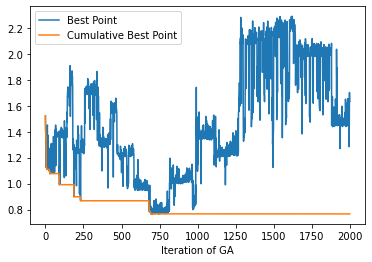
\includegraphics[width=0.7\textwidth]{Post_11_ga1}
\caption{GA Solving $f(x)$ | $p_{mut}=0.01$, $N=10$, $M=2000$}
\end{figure}

\section{Solving A Multi-Fidelity GP Model with GAs}

We now move on from the toy model to a harder one, maximizing the likelihood of a multi-fidelity gaussian process model (GP). You don't need to know why, but the likelihood of a multi-fidelity GP model for given hyperparamters $\theta$ will be as follows:

\begin{align*}
log(L)=-0.5log(det(K_y))-0.5Y^T(K_y)^{-1}Y-N/2log(2\pi)-0.5(\theta-\bar{\theta})^T \Sigma^{-1} (\theta-\bar{\theta})
\end{align*}

\begin{align*}
k_y=K(X,X)+\sigma_n^2
\end{align*}

\vspace{5mm}

Which differs slightly from our usual $L(\theta)$ equation from Post 2 via the $-0.5(\theta-\bar{\theta})^T \Sigma^{-1} (\theta-\bar{\theta})$ term. This term represents a prior normal distribution (or rather the log of that distribution) for the hyperparameters. The model itself looks very much like the GP we used previously:

\begin{align*}
\mu(x^*)=K(x^*,X)^T(K_y)^{-1}Y
\end{align*}

\begin{align*}
\sigma^2(x)=k(x^*,x^*) - K(x^*,X)(K_y)^{-1}k(x^*,X)^T
\end{align*}

\vspace{5mm}

The major difference is the kernel matrix $K(x,x')$ which is as follows:

\begin{align*}
K(x,x')=K_0(x,x')+\{IS \neq 0, IS = IS'\}K_l(x,x')
\end{align*}

\vspace{5mm}

Where $K_0(x,x')$ is a squared exponential kernel for regression over a 'primary' information source (a really good model for example) and $K_l(x,x')$ is the kernel for data from $l$ information source (a less good model for example). We will solve the problem $\theta^* = argmin -log(L(\theta))$ for a given set of data of $|l|=3$ sources of information using the GA developed above. We will be going into how this work in future posts (because it is also a big part of a new project I am working on) but suffice to say it'll be interesting. Here is the result using l-BFGS-B optimizer which approximates its own Hessians and gradients versus the same model for a GA.

\begin{figure}[h]
\centering
\subfloat[][L-BFGS-B]{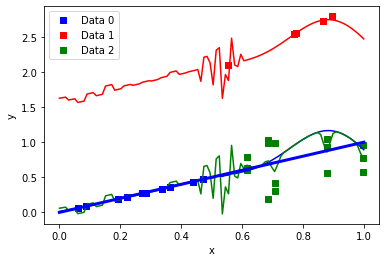
\includegraphics[width=0.35\textwidth]{Post_11_lbfgsb}}
\subfloat[][GA]{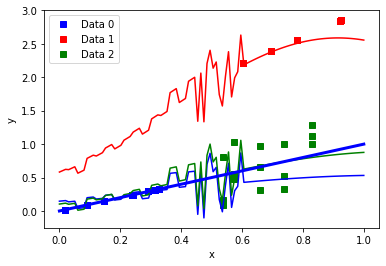
\includegraphics[width=0.35\textwidth]{Post_11_ga2}}
\caption{Multi-Fidelity GP}
\end{figure}

\vspace{5mm}

Also noting the convergence results of the GP.

\begin{figure}[h]
\centering
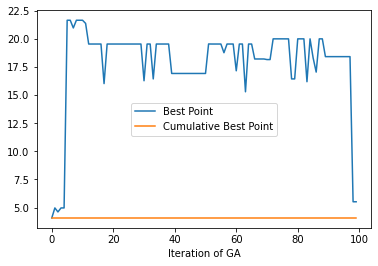
\includegraphics[width=0.7\textwidth]{Post_11_ga3}
\caption{GA Solving Multi-Fidelity GP | $p_{mut}=0.01$, $N=10$, $M=100$}
\end{figure}

\vspace{5mm}

I actually didn't realize until I was running the GA that \textbf{it takes forever}. Note from Figure 3 we are using $N=10$ per round of $M=100$ generations. This means $M*N$ calculations need to be made with the matrix inverse to calculate $-log(L(\theta))$. Funny enough, the best solution was found almost immediately and doesn't look too different from the L-BFGS-B solution (note to self, change bounds of GA to be in line with L-BFGS-B haha). This proves an important point, that GAs are very useful for cheaply solved functions like the toy function from Part 1, but not for expensive ones. This actually is a big theme in optimization, that problem complexity may determine which method you can use. 

\vspace{5mm}

Well that's all folks. This time I'll tell you what we'll be working on next week. It'll be a continuation of this work on the multi-fidelity GPs!

\end{document}